\documentclass{beamer}
\usepackage[utf8]{inputenc}
\usepackage[T1]{fontenc}
\usepackage{graphicx}
\usepackage{tcolorbox}
\usepackage{hyperref}
\hypersetup{
    colorlinks=true,
    linkcolor=pink,
    urlcolor=cyan,
    urlbordercolor=cyan,
}
\graphicspath{ {./images/} }

\usetheme{Arguelles}

\title{Tutorial 5}
\subtitle{CS3241 Computer Graphics (AY23/24)}
\date{\today}
\author{Wong Pei Xian}
\institute[]{\email{e0389023@u.nus.edu}}

\begin{document}

\frame[plain]{\titlepage}

\section{Lecture 6}

\begin{frame}
    \frametitle{Summary}

    \begin{itemize}
        \item Clipping 
        \begin{itemize}
            \item Cohen Sutherland (Line Clipping)
            \item Polygon Clipping
            \item Simple early acceptance/rejection
        \end{itemize}
        \item Rasterization of Line Segments
        \begin{itemize}
            \item Digital Differential Analyzer
            \item Bressenham's Algorithm
        \end{itemize}
        \item Culling
        \begin{itemize}
            \item Painter's Algorithm (Depth sorting)
            \item Back-face culling
            \item Image space (Ray-tracing, closest polygon per pixel)
            \end{itemize}
    \end{itemize}

\end{frame}

\begin{frame}[plain,standout]
    \AlegreyaExtraBold \LARGE
    Tutorial 5
\end{frame}

\section{Question 1}

\begin{frame}
    \frametitle{Question 1}
    We want to scan-convert (rasterize) the curve \textcolor{teal}{$y = x^2 / 100$} from the pixel locations $(0, 0)$ to $(200, 400)$. 
    Assume there is a function \texttt{write\_pixel(x, y, color)} to set the color of a pixel at location $(x, y)$. 
    The curve should be drawn as the thinnest possible but not broken. 
    Write a C program fragment to draw the curve. 

    \vspace{1em}
    
    \textit{You are allowed to use floating-point operations, the \texttt{round()} function, and even the square-root function \texttt{sqrt()}.}
\end{frame}

\begin{frame}
    \frametitle{Which algorithm?}

    \textbf{Floating Point ops allowed} $\rightarrow$ Digital Differential Analyzer

    \begin{equation*}
        m = \frac{dy}{dx} = \frac{y_e - y_0}{x_e - x_0}
    \end{equation*}

    Obtain $m = \frac{dy}{dx} = \frac{d}{dx} (x^2/100) = 50x$.

    \begin{center}
        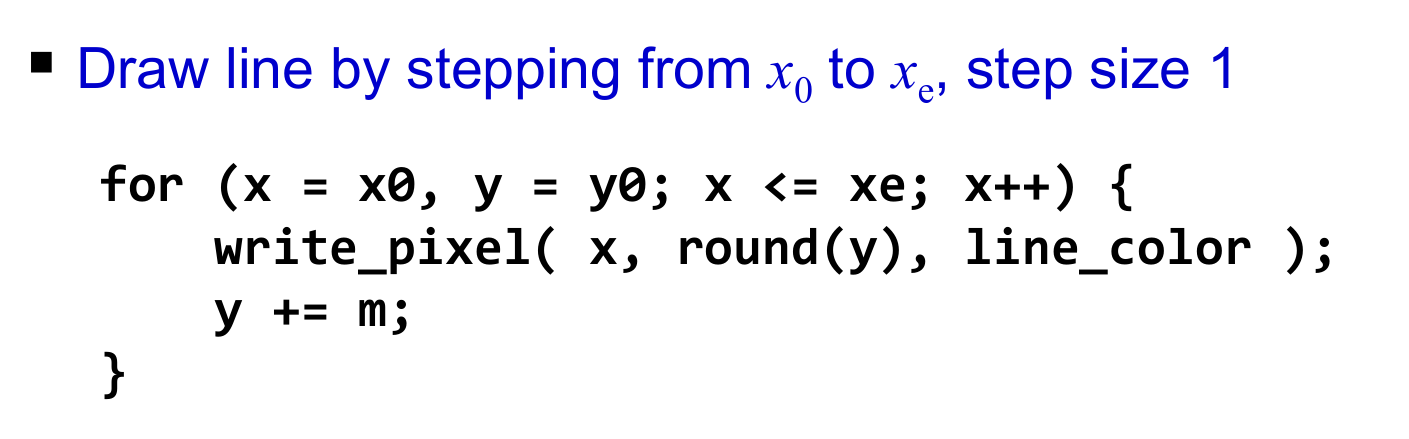
\includegraphics[scale=0.4]{dda-algo.png}
    \end{center}

\end{frame}

\begin{frame}
    \frametitle{Do we actually need to \texttt{y += m}?}

    No. We already know the relationship between $y$ and $x$.

    \vspace{1em}

    \begin{tcolorbox}
        \texttt{for (int x = 0; x <= xe; x++) \\
        \hspace{1em} int y = x*x /100;\\
        \hspace{1em} write\_pixel(x, y, color);}
    \end{tcolorbox}

\end{frame}

\begin{frame}
    \frametitle{Inherent problem in vanilla DDA}

    \begin{center}
        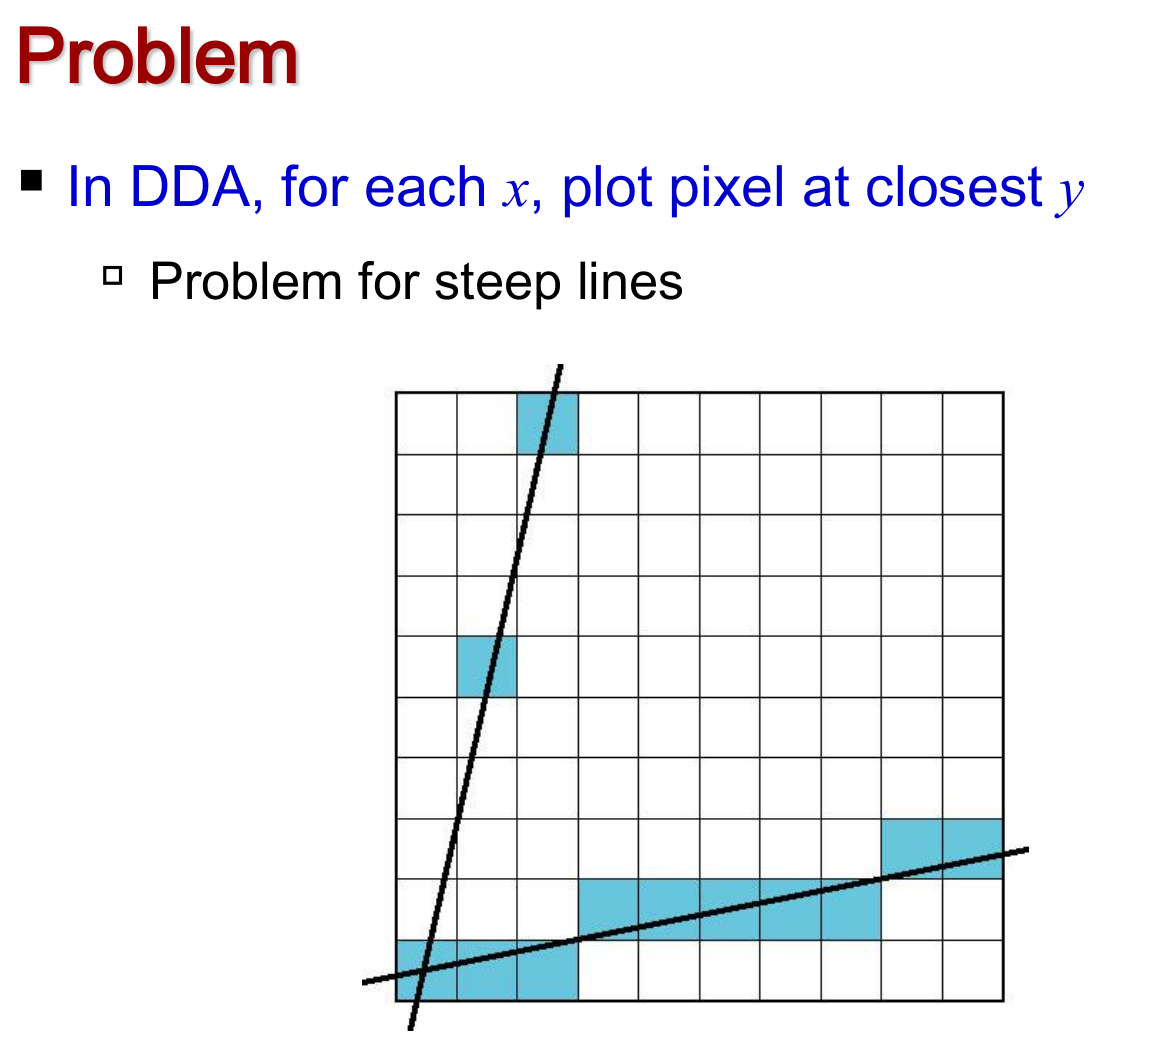
\includegraphics[scale=0.3]{dda-problem.png}
    \end{center}

    This is where the $m = \frac{dy}{dx}$ comes in handy! 
    We use it to identify when to swop roles of $x$ and $y$.

\end{frame}

\begin{frame}
    \frametitle{Solving this problem}

    \begin{center}
        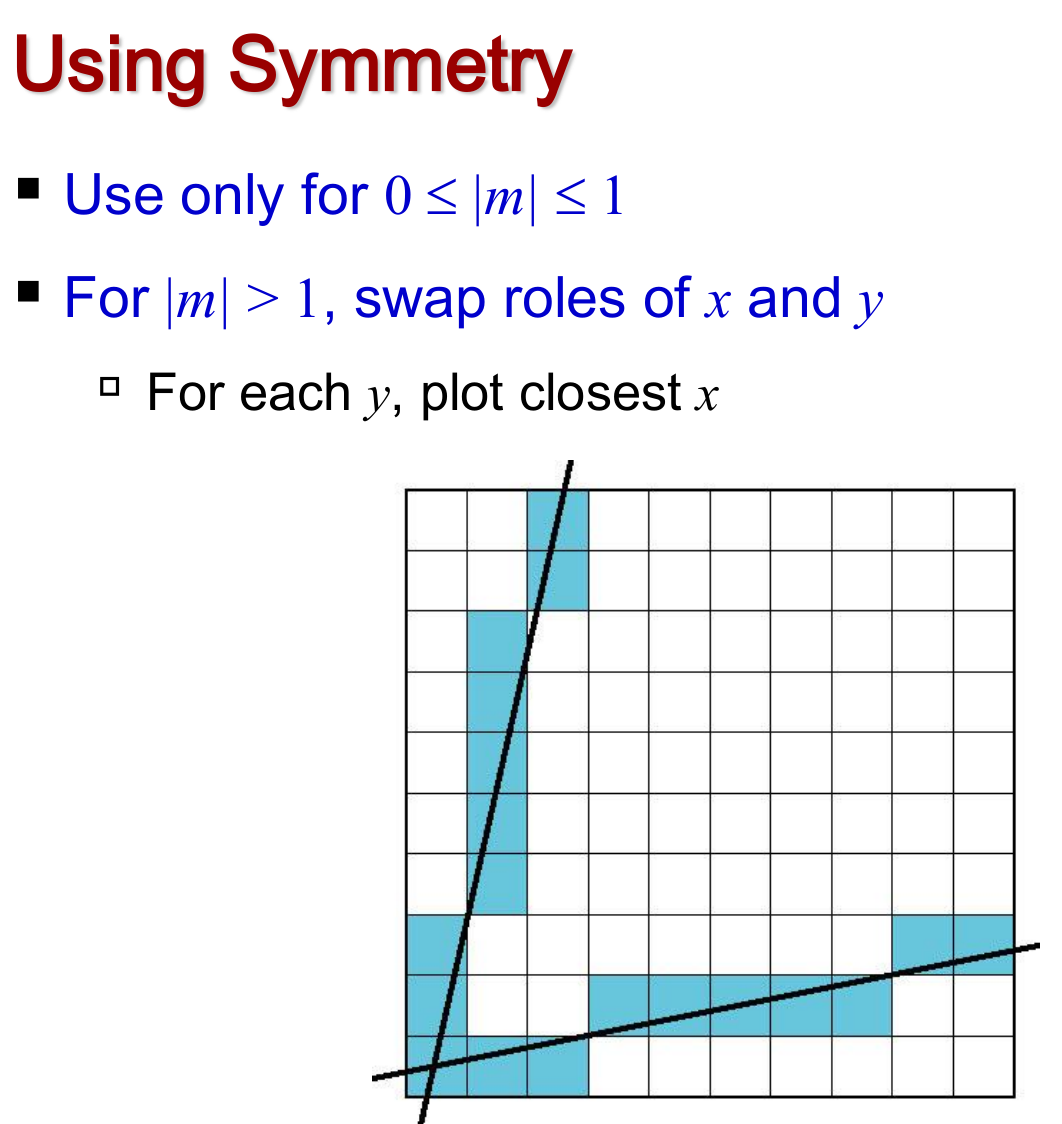
\includegraphics[scale=0.3]{dda-soln.png}
    \end{center}

    We use it to identify when to swop roles of $x$ and $y$.
    
    \begin{equation*}
        m = \frac{x}{50} > 1 \Rightarrow \textcolor{magenta}{x > 50}
    \end{equation*}

\end{frame}

\begin{frame}
    \frametitle{Complete Solution}

    

\end{frame}

\section{Question 2}

\begin{frame}
    \frametitle{Question 2}
    How do you scan convert a \textcolor{teal}{circle} \textcolor{magenta}{without using any floating-point operations}? 
    Assume that the circle center has integer pixel coordinates and its radius is an integer. 
    Assume the entire circle is inside the window. 
    Complete the following program fragment. 

    \vspace{1em}
    
    \textit{You are allowed to use a few floating-point operations in the initialization or setup.}
\end{frame}

\begin{frame}
    \frametitle{Question 2}

    \begin{center}
        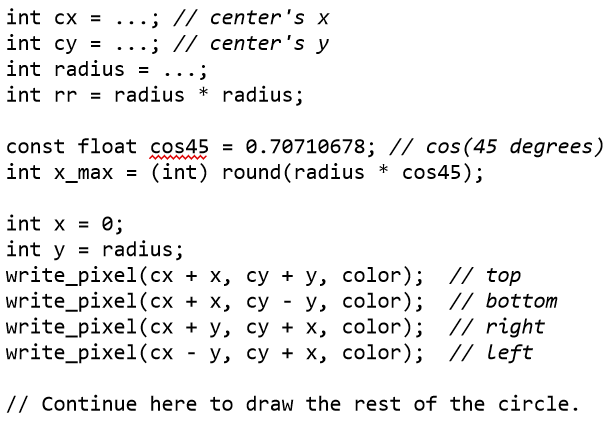
\includegraphics[scale=0.8]{q2.png}
    \end{center}

\end{frame}

\begin{frame}
    \frametitle{Which algorithm?}

    \textbf{Floating Point ops NOT allowed} $\rightarrow$ Bresenham's Algorithm

    Hints in the code:
    \begin{itemize}
        \item \texttt{x\_max = (int) round(radius * cos45}: 
        \item 4 starting pixels: top bottom right left
    \end{itemize}

\end{frame}

\begin{frame}
    \frametitle{Pattern}

    \begin{center}
        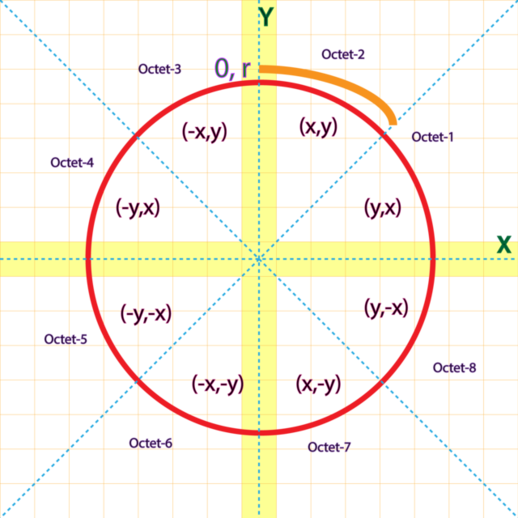
\includegraphics[scale=0.45]{bresenham-circle.png}
    \end{center}

\end{frame}

\begin{frame}
    \frametitle{Bresenham's algorithm}

    With $x = 0$ and $y = r$, we are starting at the \textbf{top}.

    \begin{tcolorbox}
        \begin{center}
            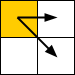
\includegraphics[scale=0.8]{bresenham-decision.png}\\

            If we have just shaded the yellow pixel \texttt{(cx + 0, cy + radius)}, 
            for \texttt{cx+1} how do we know which pixel to shade?\\
        \end{center}
    \end{tcolorbox}

    \vspace{1em}

    Don't try differentiating $y^2 + x^2 = r^2$: even with assumptions on the values of
    y and x it will get clunky and involve \texttt{sqrt} which is prohibited.

\end{frame}

\begin{frame}
    \frametitle{Bresenham's \textbf{Circle} algorithm}

    We know that in a \textbf{perfect circle}, $y^2 + x^2 - r^2 = 0$.\\

    Hence for a given $y$, the closer the value of $\mid y^2 + x^2 - r^2 \mid$ to 0, 
    the closer it is to the perfect circle.

    \begin{center}
        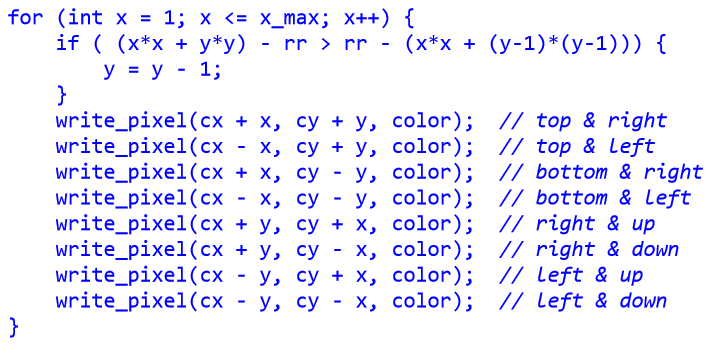
\includegraphics[scale=0.6]{q2-soln.png}
    \end{center}

    Observe the symmetry.

\end{frame}

\section{Question 3}

\begin{frame}
    \frametitle{Question 3a}
    What could be the problems with the rasterization of a very thin triangle?

\end{frame}

\begin{frame}
    \frametitle{In context of rasterization...}

    The main problem we've seen is this one:

    \begin{center}
        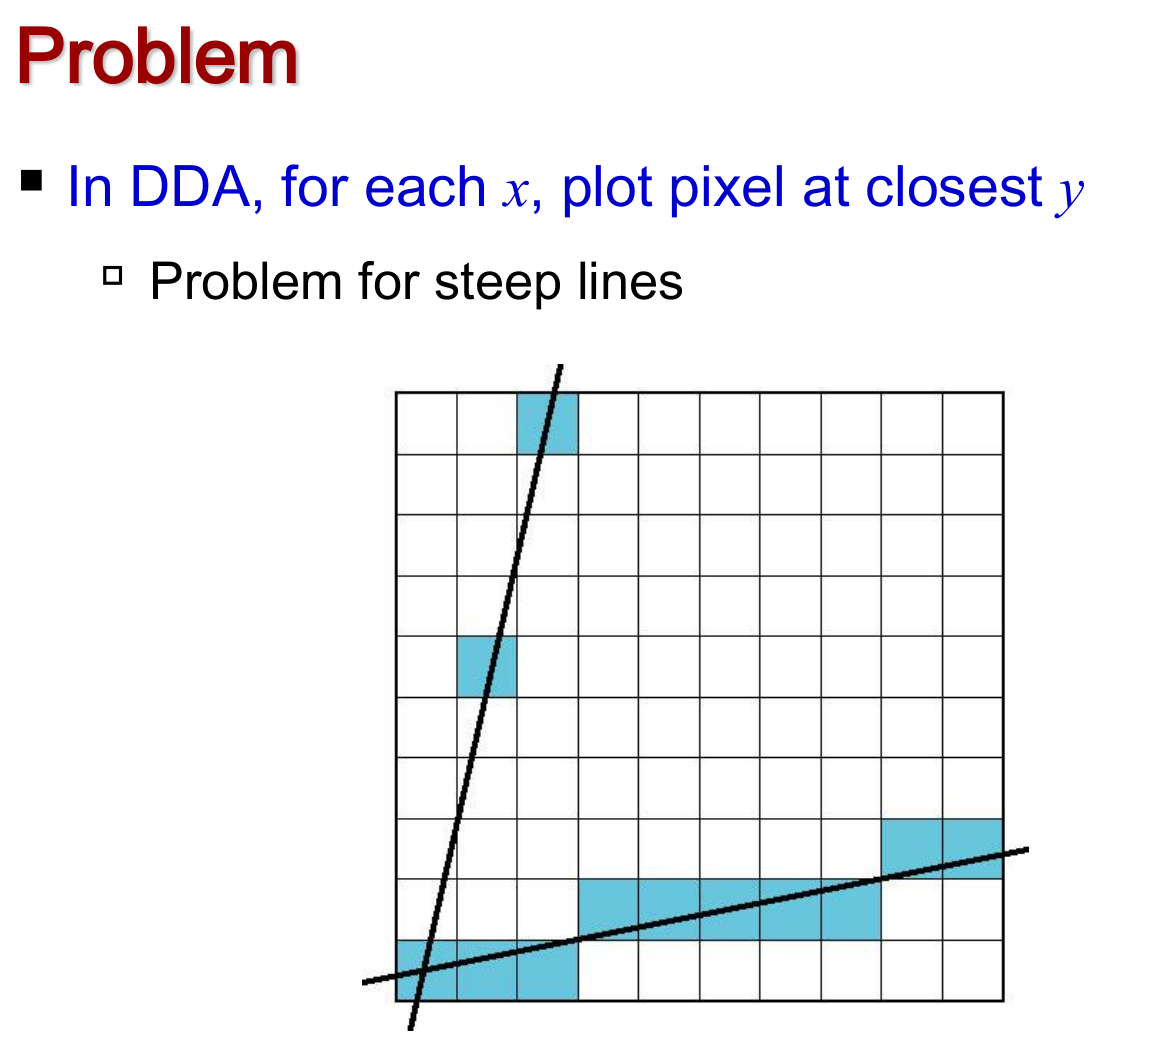
\includegraphics[scale=0.3]{dda-problem.png}
    \end{center}

\end{frame}

\begin{frame}
    \frametitle{In context of rasterization...}

    Notice this would happen with thin triangles too.

    \begin{center}
        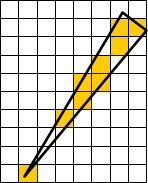
\includegraphics[]{thin-tri.png}
    \end{center}

\end{frame}

\begin{frame}
    \frametitle{Question 3b}

    Would it still be a problem if the thin triangle is part of a triangle mesh?

    \vspace{1em}

    No, all the spaces will be filled up.

    \begin{center}
        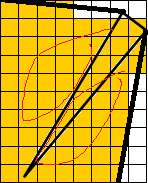
\includegraphics[scale=0.8]{thin-tri-mesh.png}
    \end{center}

\end{frame}

\section{Question 4}

\begin{frame}
    \frametitle{Question 4a}
    The following image shows the rendering of a green rectangle and a red rectangle in 3D space. 
    In the overlap area of the two rectangles, there is some rendering artifact caused by z-fighting. 
    What do you think z-fighting is? What is the cause of z-fighting in this example? 

    \begin{center}
        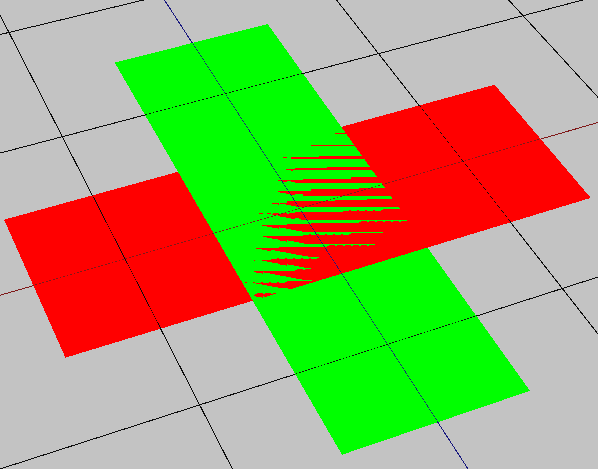
\includegraphics[scale=0.25]{z-fighting.png}
    \end{center}
\end{frame}

\begin{frame}
    \frametitle{z-fighting}

    \begin{itemize}
        \item 2 or more primitives have \textbf{very similar distances to camera}
        \item Near similar or \textbf{identical} values in the z-buffer.
        \item The fragment to rasterize is chosen \textbf{randomly} between the fighting fragments.
    \end{itemize}

\end{frame}

\begin{frame}
    \frametitle{Question 4b}

    When you are setting up a view volume, what can you do to minimize the chance of z-fighting? 

    \vspace{1em}
    \textit{i.e. how to \textbf{reduce the likelihood of the primitives having identical values}}

\end{frame}

\begin{frame}
    \frametitle{Minimizing z-fighting}

    Since z-buffer values have to be between $[0, 1]$, the bottleneck (for the number of possible z-buffer values)
    is the \textbf{precision/bit count} of the floating point value (16, 32, or 64).

    \begin{enumerate}
        \item Increase the \textcolor{magenta}{precision} (number of bits) of z-buffer value.
        \item Decrease the \textcolor{teal}{distance between the near and far} plane (how is z-buffer value calculated?)
        \begin{itemize}
            \item $[\text{near}, \text{far}] \mapsto [0, 1]$
            \item range of possible values with same z-buffer value: 
                $[\text{near}, (\text{near} - \text{far})/(2^N)]$
        \end{itemize}
    \end{enumerate}

\end{frame}

\begin{frame}[plain,standout]
    \AlegreyaExtraBold \LARGE
    Attendance taking
\end{frame}

\ThankYou
\begin{frame}[plain,standout]
    Thanks! Get the slides here after the tutorial.\\
    \vspace{2em}
    \scalebox{3}{\faGithub}\par\bigskip
    \url{https://trxe.github.io/cs3241-notes}
\end{frame}

\end{document}